\begin{center}
  \Large
  \textbf{AUTHOR'S BIOGRAPHY}
\end{center}

\addcontentsline{toc}{chapter}{AUTHOR'S BIOGRAPHY}

\vspace{2ex}

\begin{wrapfigure}{L}{0.3\textwidth}
  \centering
  \vspace{-3ex}
  % Ubah file gambar berikut dengan file foto dari mahasiswa
  %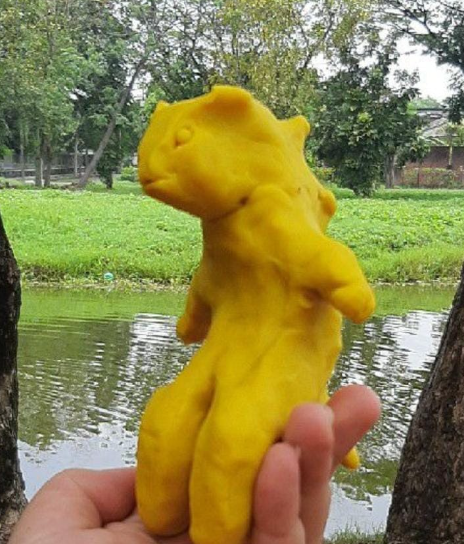
\includegraphics[width=0.3\textwidth]{figures/yellow.png}
  
\includegraphics[width=0.3\textwidth]{figures/profile-silhuette.jpg}
  \vspace{-4ex}
\end{wrapfigure}

% Ubah kalimat berikut dengan biografi dari mahasiswa
\name{}, born on the day he was born, was a creature with many interests.
%\lipsum[1-2]
He began his journey on exploring computer science and engineering when he was in his third year of middle school.
He encountered a random C programming language book in a bookstore, bought it, read it, and created his first hello world right after.

His training arc started in high school. 
Due to an unknown reason, his homeroom teacher forced him to enroll in the high school's mathematics olympiad team.
As he was a pushover back then, he just followed what his teacher said.
Fortunately, the math teacher didn't really want to teach olympiad level math, and recommended him to try informatics olympiad instead.
That's how he met his master who taught him the competitive programming 101 and robotics.

Fast-forward to his university year, he enrolled in an autonomous surface vehicle student team.
There, he learned the art of multidisciplinary teamwork and a lot of failure analysis technique. 
He was once tasked on developing a computer vision system for a robot. This final project was actually
a continuation from that system.

Most of his activities during the making of this final project includes listening Trash Taste podcast,
playing saxophone, and watching v-tubers. 
Honestly, most of the work here is done by the red computer in B201 lab.
With model training lasts around a day for each model, he can't help but spend those idle time to things other than this final project.
Therefore, let's just forget about \name{} because that red computer is the real hero for this one.

%\lipsum[1]

%\lipsum[2]
